\chapter{基于深度相机模型形变捕捉}
要构建模型的形变子空间,除了静态三维模型,
还需要一些形变后的模型,即形变关键帧作为输入。
本章描述了一个以静态模型和深度视频为输入的形变捕捉算法。
在捕捉步骤中,操作者会带着特定颜色的手套,在深度相机前摆弄物体,使得物体发生形变。
该算法会优化模型的形变参数,使得模型的形状和相机采集的物体形状尽量吻合,
从而得到形变后的模型。
本文会从捕捉到的形变中选取若干成为形变关键帧,作为形变子空间构建的输入。
本章接下来就会阐述该算法的技术细节。

\section{基于手部信息的模型初始位姿确定}

 类似于三维重建步骤中的相机位姿估计,
 在形变步骤中,对于每一帧深度图像,本文仅计算模型和上一帧的相对形变。
 因此,在捕捉形变之前,需要得知模型的初始位置。
 在本文的形变捕捉流程中,操作者需要用手持物。
 所以物体必然位于手的附近,所以本文设计了一个借助手部信息确定模型的初始位置与朝向的算法。
 本位所采用的确定物体初始位姿的算法可主要分为三个步骤:分割手部点云、分割物体点云、模型对齐。
 本节接下来就会详细描述这一流程。

\subsection{手部点云分割}
由于本文是借助手部点云的位置寻找物体的点云,
所以需要在输入的点云中分割出属于手的部分。
本章就将描述一种基于RGBD图像的点云分割算法。

分割手部点云阶段的输入是RGBD图像,输出为手部的像素坐标的集合。
RGBD图像即除了RGB三个颜色通道外,还有一个深度通道
记录了对应点距离相机的距离,可以理解为RGB图像加上深度图像。
Kinect分别通过色彩传感器和深度传感器获得RGB图像和深度图像,
由于两个传感器的相对位置被事先标定过,
所以Kinect的SDK提供了将RGB图像映射到深度图像的接口,
映射后的RGB图像的像素和深度图像的像素一一对应。
为了描述方便,本文中提到的RGB图像均指映射后的RGB图像。
如图\ref{finding_hand}所示,
分割手部点云阶段可主要分为颜色过滤、深度过滤、寻找最大连通域三个步骤。

首先,本文会根据筛选出颜色和指定颜色相近的像素点。

\begin{algorithm}
    \fangsong
    \caption{分割手部点云}
    \label{alg_seg_hand}
    \begin{algorithmic}[1]
        \Require RGB图像$\mathbf{C_i}$,深度图像$\mathbf{D_i}$,颜色集$\mathbf{C_{hand}}$
        \Ensure 手部像素集合$\mathbf{P_{hand}}$
        \State $\mathbf{V_i} \gets DepthConvert(\mathbf{D_i})$ \Comment{将深度图转换为顶点图}
        \State $\mathbf{P_{hand}} \gets \mathbf{\emptyset}$
        \For {$\forall\mathbf{u} \in \mathbf{U_{image}}$}\Comment{找出所有与指点颜色集合中的颜色相近的像素}
            \For {$\forall\mathbf{c} \in \mathbf{C_{hand}}$}
                \If{$|\mathbf{C_i}(u) - \mathbf{c}| \leq thd_{color}$}
                   \State $\mathbf{P_{hand}} \gets \mathbf{P_{hand}} \bigcup \{\mathbf{c}\}$
                \EndIf
            \EndFor
        \EndFor
    \end{algorithmic}
\end{algorithm}

\begin{figure}[h]
    \centering
    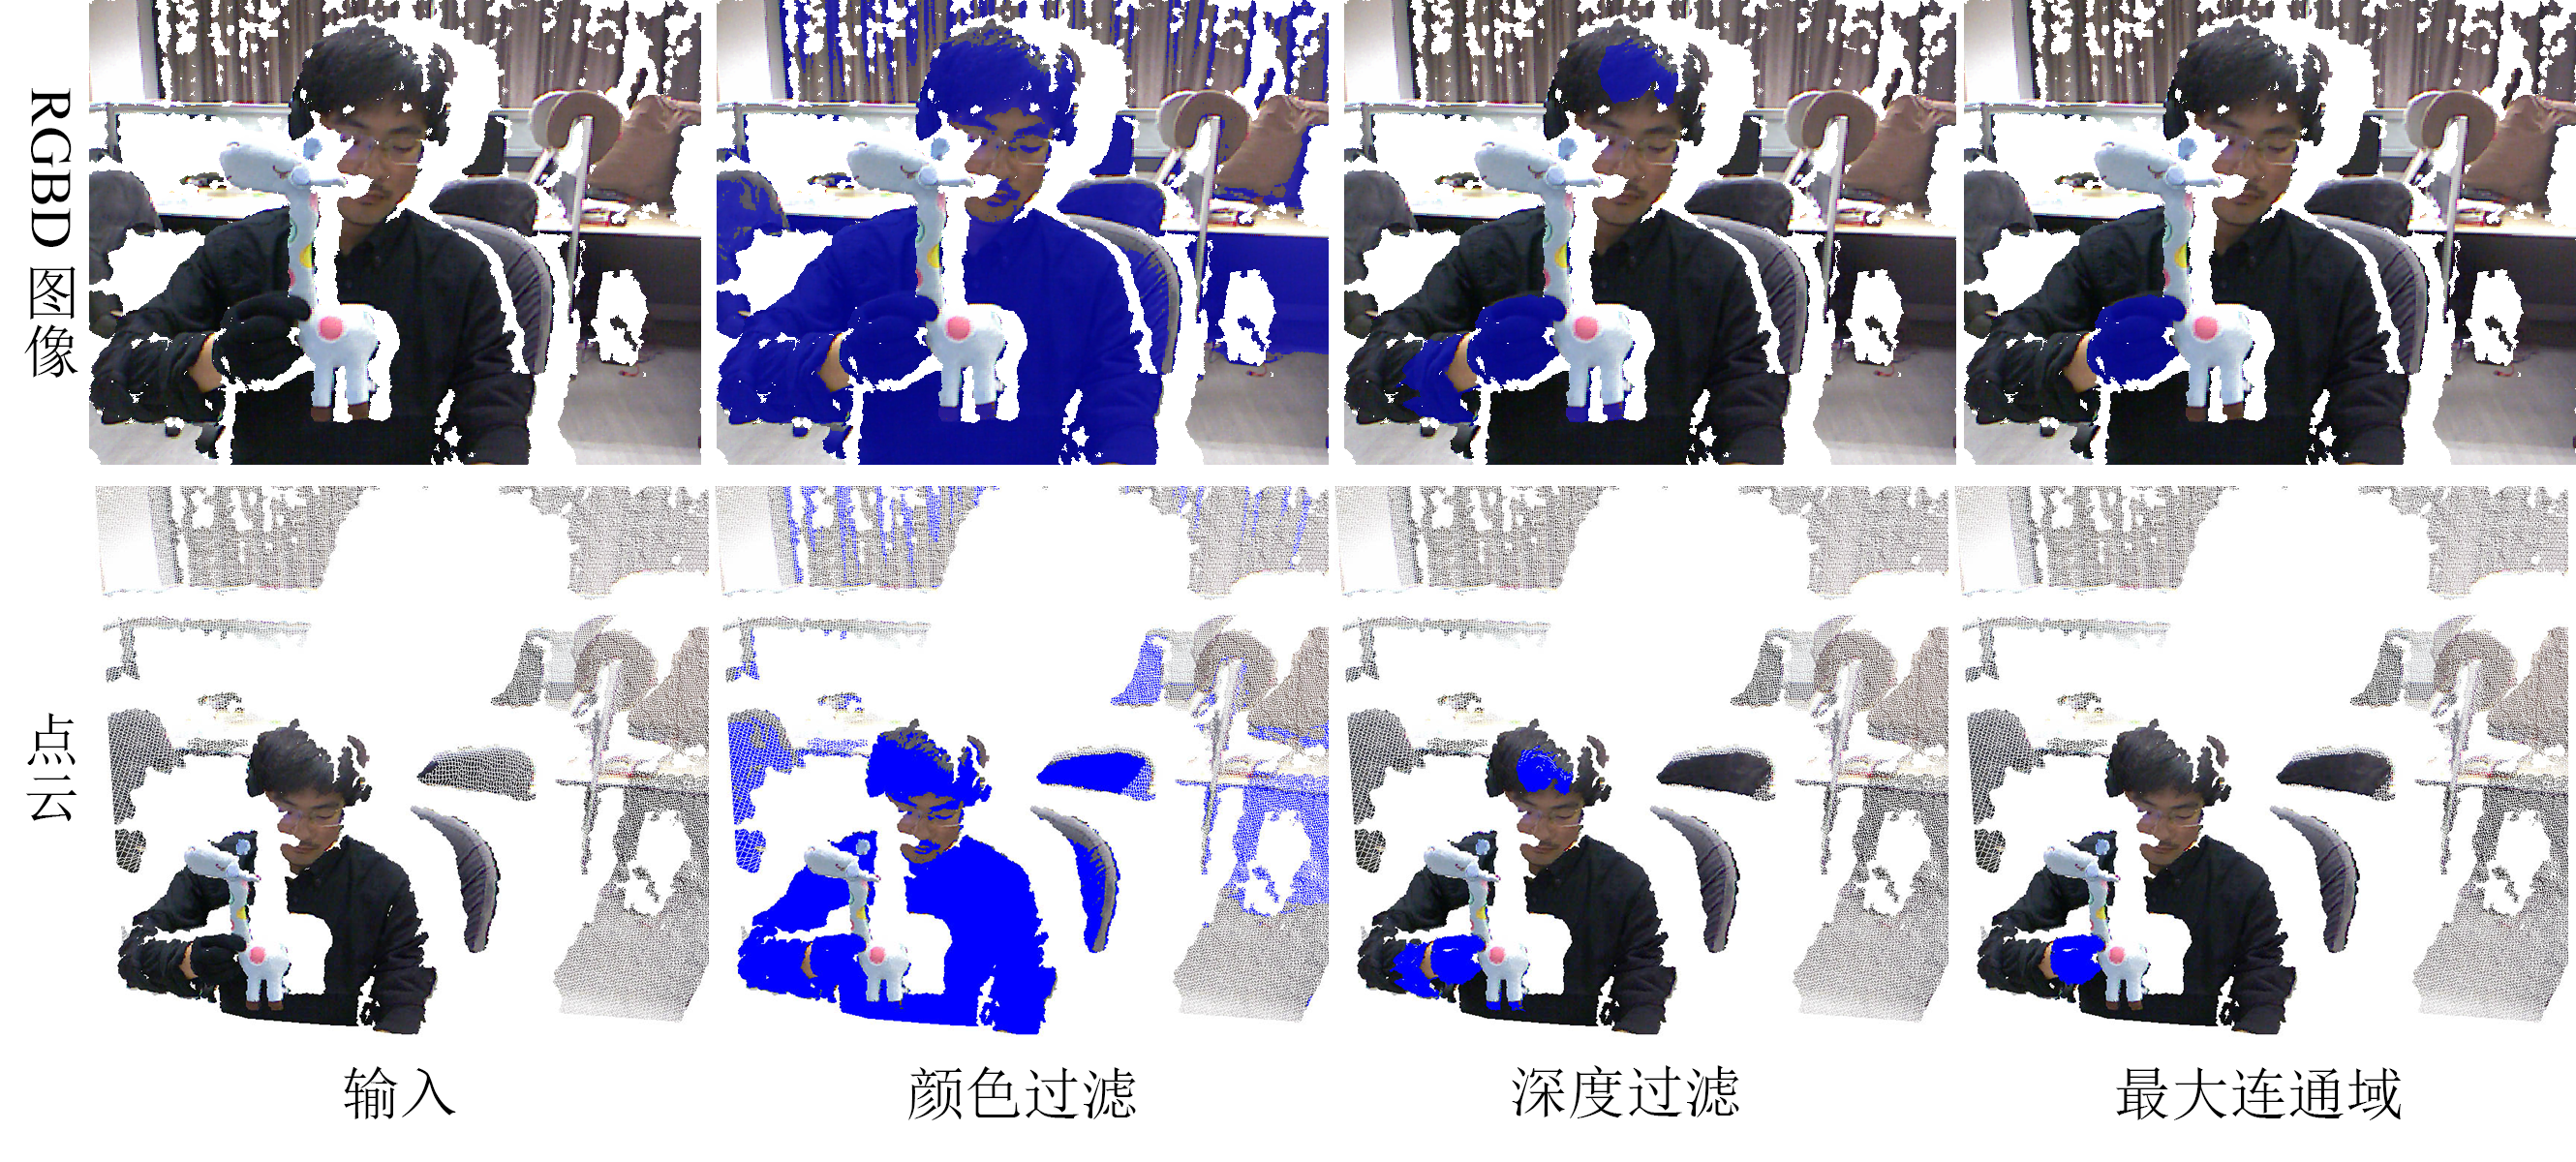
\includegraphics[width = \textwidth]{./Pictures/FindingHand.png}
    \caption{手部点云分割流程}
    \label{finding_hand}
\end{figure}
\subsection{物体点云分割}
\subsection{模型对齐}

\section{基于深度视频的形变捕捉}
\subsection{形变的参数化描述}
\subsection{形变参数优化}

\section{本章小结}